
En este capítulo se definirán los conceptos  o fundamentos de instrumentación estructural, sensores inteligentes y adquisición de datos, necesarios para llevar a cabo esta investigación.

\section{Estructuras civiles}

\subsection{Características generales}

Una estructura se refiere a un sistema de partes o elementos que se interconectan para cumplir una función es específico. En el caso de la ingeniería civil, suelen ser miembros que se utilizan para soportar una carga. Algunos ejemplos importantes son los edificios, los puentes y las torres; y en otras ramas de la ingeniería, son importantes las corazas de barcos y aviones, los sistemas mecánicos y las estructuras que soportan las líneas de transmisión eléctrica \citep{hibbeler1997structural}.

\subsection{Tipos de estructuras}

Según \citet{hibbeler1997structural}, cada sistema está formado por uno o varios de los cuatro tipos básicos de estructuras: 

\begin{itemize}
    \item Celosías.
    \item Cables y arcos.
    \item Armazones.
    \item Estructuras de superficie.
\end{itemize}

En general, estos elementos suelen soportar cargas, pueden ser estacionarios y también estar restringidos. Sus diferencias suelen basarse en la cantidad de fuerzas a las que están sujetos estos elementos en un instante dado.

La combinación de estos elementos y los materiales que los componen es lo que se denomina un sistema estructural. Estos sistemas, aunque sean pasados por alto, son utilizados diariamente por industrias y personas, siendo elementos claves en el desarrollo y progreso de la civilización actual.

\subsection{Comportamiento de las estructuras civiles}

La gran mayoría de los sistemas cuentan con una respuesta dinámica y estática. Ambas respuestas permiten conocer el comportaiento completo del sistema en estudio ante distintas entradas o en diferentes situaciones. Al estudiar el comportamiento estructural se encuentra una extensa literatura tanto para el estudio dinámico como para el régimen estático, recopilándose lo siguiente:

\begin{itemize}
    \item{Respuesta estática}: En la ingeniería civil toda estructura se diseña para que se encuentre en reposo cuando actúan sobre esta fuerzas externas, es decir, la estructura en conjunto debe cumplir con las condiciones de equilibrio, siendo la fuerza y el momento resultanto sobre esta igual a cero en todo momento. Para describir estas condiciones de equilibrio se cuentan con herramientas matemáticas que proporcionan las condiciones necesarias para su cumplimiento. Estas ecuaciones permiten la resolución estática de la estructura, la cual permite determinar el valor de todas las incógnitas estáticas de interés \citep{basset2014analisis}.
    
    \indent Cuando las fuerzas que actúan sobre la estructura pueden calcularse a partir de las ecuaciones de equilibrio, se tiene una estructura en equilibrio y se denonima estructura estáticamente determinada. En caso de tenerse más fuerzas desconocidas que ecuaciones de equilibrio se habla de una estructura estáticamente indeterminada.

        \begin{itemize}
            \item Rigidez: Uno de los parámetros más importantes dentro de la respuesta estática es la rigidez. Esta se define como la propiedad que tiene un elemento estructural de soportar la deformación o deflección al estar bajo la acción de una fuerza o carga. Una medida de la rigidez viene dada por el Módulo de Young; esta es una constante del material y es independiente de la cantidad de material.
        \end{itemize}

    \item{Respuesta dinámica}: La dinámica estructural se encarga de estudiar el efecto que tienen cargas dinámicas sobre el sistema. La respuesta ante estos eventos, como pueden ser sismos, vientos, equipos mecánicos, paso de vehículos o personas, se denomina respuesta dinámica \citep{hurtado2000}. Además, la respuesta dinámica permite caracterizar algunos parámetros de gran interés para estudiar su comportamiento conocidos como parámetros modales. Estos parámetros surgen al estudiar las ecuaciones diferenciales que describen el movimiento de la estructura, partiendo de un modelo idealizado simple de masa concentrada como el de la Figura \ref{fig:masa_estructural}.
    
    \begin{figure}[H]
        \centering
        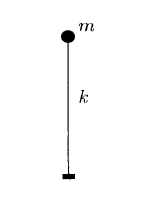
\includegraphics[width = 0.25\textwidth]{imagenes/cap1_marcoteo/modelo_masa_simple.png}
        \caption{Modelo de masa concentrada de 1 grado de libertad (Fuente: Introducción a la Dinámica Estructural).}
        \label{fig:masa_estructural}
    \end{figure}

    La dinámica de este modelo puede describirse utilizando la ecuación diferencial de movimiento:

    \begin{equation} \label{eq:vib_lib}
        m\ddot{u} + f_R(t) = p(t)
    \end{equation}

    La ecuación \ref{eq:vib_lib} se conoce como ecuación de vibración libre sin amortiguamiento. Donde $p(t)$ representa las cargas dinámicas y $f_R(t)$ la fuerza de restitución propia de un material elástico.  Esta ecuación es una ecuación diferencial de coeficientes constantes, que consta de una solución homogénea más una solución particular. La solución homogénea será la respuesta de la estructura a la vibración libre, es decir, si la masa de la Figura \ref{fig:masa_estructural} se deja oscilar libremente.

    Se sabe que una ecuación de este tipo tendrá una solución como:

    \begin{equation} \label{eq:sol_equ_dif}
        u = A.sin\omega t + B.cos\omega t
    \end{equation}

    La ecuación \ref{eq:sol_equ_dif} contiene información relevante para la caracterización dinámica de la estructura. Esta caracterización parte del estudio de los parámetros modales de la misma.

    Entre estos parámetros modales se encuentran: 
        \begin{itemize}
            \item Frecuencia natural: Toda estructura física tiene asociada una frecuencia de vibración natural. Las máquinas, los puentes, los edificios; todas estas estructuras vibran u oscilan al ser perturbadas o removidas de su estado de reposo inicial. Es una propiedad es intrínseca del sistema y depende de su masa, rigidez y amortiguamiento. Todas tienen al menos una frecuencia natural y es posible que tengan múltiples frecuencias de resonancia \citep{irvine2000introduction}. 
            
                Se suele calcular la frecuencia natural de resonancia de un sistema libre usando:

                \begin{equation}
                    f =  \frac{1}{\sqrt{\frac{k}{m}}}
                \end{equation}

            \item Amortiguamiento: Toda estructura comienza a oscilar una vez es removida de su estado de reposo o equilibrio, sin embargo, ese movimiento no es perpetuo. El amortiguamiento se define como la capacidad de disipación de energía que posee la estructura bajo excitaciones externas. Las soluciones a la ecuación \ref{eq:vib_lib}, al añadir el amortiguamiento de tipo viscoso, arrojan 3 posibles casos:
                \begin{enumerate}
                    \item Sistema críticamente amortiguado: El sistema no vibra.
                    \item Subamortiguado o amortiguado subcrítico: Caso más común por la naturaleza de los materiales utilizados en las estructuras. La respuesta del sistema decae con el tiempo de forma exponencial, como se puede ver en la Figura \ref{fig:resp_subamorti}. 
                    
                    \begin{figure}[H]
                        \centering
                        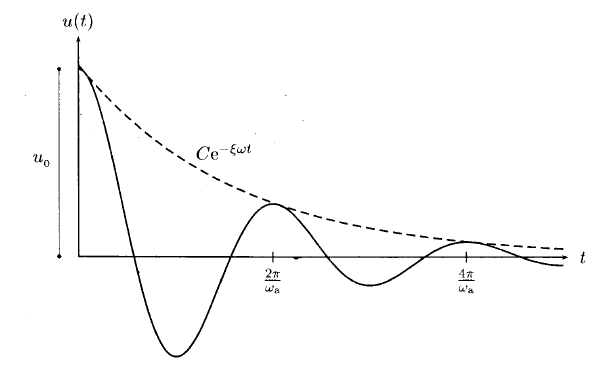
\includegraphics[width = 0.7\textwidth]{imagenes/cap1_marcoteo/respuesta_sist_subamorti.png}
                        \caption{Respuesta ante vibración libre en sistema Subamortiguado (Fuente: Introducción a la Dinámica Estructural).}
                        \label{fig:resp_subamorti}
                    \end{figure}

                    \item Sobreamortiguado: Nunca se encuentra esta respuesta en sistemas estructurales por los materiales utilizados.
                \end{enumerate}
            
        \end{itemize}        
\end{itemize}

\subsection{Respuesta en frecuencia}

    Incluir?

\subsection{Daño en estructuras}

El daño a una estructura civil o mecánica puede definirse como todo cambio en las propiedades materiales o geométricas del material que llegan a afectar de forma adversa la confiabilidad y el desempeño actual o futuro del sistema. Por tanto, el daño es una comparación entre el sistema en cuestión en 2 instantes de tiempo distintos \citep{farrar2007introduction}. Estos efectos adversos pueden ser, en el caso estructural, desplazamientos, estrés indeseado en un elemento o vibraciones estructurales indeseadas \citep{chen2018}.

Toda estructura civil, como puentes y edificios, acumulan daño de forma continua a medida que están en servicio y transcurre su vida útil. Este daño puede manifestarse como fracturas, fatiga, socavaciones o desprendimiento del concreto. El daño que no sea detectado puede conducir a una falla estrcutural que a su vez ocasione pérdidas humanas. Por tanto, es imperativo y necesario detectar el daño en una estrcutrura tan pronto como sea posible, \citep{chen2018}.

Entre algunos de los factores que influyen del deterioro de una estructura se encuentran:
    
        \begin{itemize}
            \item Proceso de degradación natural de los materiales.
            \item Corrosión del acero de refuerzo.
            \item Evento sísmico, incendios o condiciones de guerra.
            \item Carga por encima del límite de diseño.
        \end{itemize}
    
Las escalas de tiempo y de extensión del daño son diversas. Por ejemplo, el deterioro por el paso del tiempo bajo ciertas condiciones climáticas es muy lento comparado al daño causado por un evento catastrófico.

\subsection{Principios de la Sismoresistencia}

Una edificación sismorresistente es aquella que está diseñada y construida para soportar las fuerzas causadas por eventos sísmicos. Sin embargo, incluso las edificaciones diseñadas y construidas según las normas sismorresistentes pueden sufrir daños en caso de un terremoto muy fuerte, sin embargo, las normas establecen los requisitos mínimos para proteger la vida de
las personas que ocupan la edificación

Algunas de las características de una estructura sismoresistente son:

        \begin{itemize}
            \item Forma regular.
            \item Bajo peso.
            \item Mayor rigidez.
            \item Buena estabilidad.
            \item Suelo firme y buena cimentación.
            \item Materiales competentes.
            \item Capacidad de disipación de energía.
            \item Fijación de acabados e instalaciones.
        \end{itemize}

En Venezuela las estructuras deben cumplir con la Norma Venezolana COVENIN 1756:2001 (Edificaciones Sismorresistentes).

Se ha observado que al estudiar el comportamiento de las estructuras luego de un evento sísmico, es evidente que cuando se toman en cuenta las normas de diseño sismorresistente dispuestas en la ley y la construcción es debidamente supervisada, los daños estructurales resultan ser considerablemente menores que en las edificaciones en las cuales no se cumplen los requerimientos mínimos indispensables estipulados en la norma, \citep{blanco2012criterios}.

\subsubsection{Importancia de la instrumentación} La instrumentación estructural permite medir y monitorear las acciones y respuestas estructurales ante distintos eventos. Esto proporciona datos en tiempo real sobre el comportamiento dinámico y estático de la estructura, como deformaciones, aceleraciones y desplazamientos, que son fundamentales para evaluar y verificar si la estructura cumple con los criterios de diseño sismoresistente establecidos en la norma.

La instrumentación estructural ayuda a validar los modelos y suposiciones utilizados en el diseño estructural inicial. Al comparar los datos recopilados por la instrumentación durante un evento sísimco con las predicciones del modelo, es posible verificar si la estructura se comporta de acuerdo con las expectativas y si cumple con los criterios de seguridad establecidos en la normas.

Además, el monitoreo continuo de la estructura permite conocer el estado actual de la misma, tema que representa la idea principal del Monitoreo de Salud Estructural, permitiendo a los ingenieros evaluar si se sigue cumpliendo con la norma para luego tomar decisiones y actuar en pro de la seguridad de la edificación.


\section{Salud estructural}



\subsection{Definición}

\subsection{Reseña histórica}

\subsection{Línea de trabajo del Monitoreo de Salud Estructural}

\subsection{Métodos de identificación de daño}

        \subsubsection{Basado en modelo}

        \subsubsection{Basado en respuesta}

\subsection{Criterios de evaluación}

\subsection{Variables de interés}

\subsection{Consideraciones y desafíos}


